\chapter{Support Vector Machines}\label{chap:SVC}
In questo capitolo si descrive genericamente la famiglia dei modelli \emph{support vector machine} (SVM), ed in dettaglio la formulazione del modello per risolvere problemi di classificazione (\emph{support vector classifier}, o SVC). La~\cref{sec:kernel_methods} fornirà una breve introduzione ai metodi \emph{kernel} ed alla famiglia dei modelli SVM. La~\cref{sec:hard_margin_classifier} descrive la formulazione \emph{hard margin} per problemi di classificazione, che non ammette dati erroneamente classificati. La~\cref{sec:soft_margin_classifier} descrive la formulazione \emph{soft margin} per problemi di classificazione, che ammette la presenza di dati erroneamente classificati. La~\cref{sec:kernel_trick} descrive l'utilizzo del \emph{kernel} per i modelli SVC. Per concludere, la~\cref{sec:svc_limiti} descrive in generale le limitazioni dei modelli SVM.

\section{Metodi kernel}\label{sec:kernel_methods}
Possiamo suddividere gli algoritmi di apprendimento automatico in due categorie: algoritmi lineari e algoritmi non lineari. Nel primo caso, c'è un assunzione di fondo sulla tipologia di dati da trattare: si assume che la relazione tra i dati $\Vec{x}$ e le rispettive etichette $y$ sia lineare e quindi modellabile con una funzione $f(\Vec{x}) = \Vec{w}\cdot\Vec{x} + b$.
Nel secondo caso, si assume che la relazione tra $\Vec{x}$ ed $y$ non sia lineare, e quindi la funzione $f$ che la descrive sia arbitrariamente complessa.
In genere, produrre un modello lineare è relativamente facile, ma molti scenari reali esprimono relazioni non lineari. Adottare un modello lineare in questi casi porterebbe ad insufficienti capacità di generalizzazione, dovute alla troppa semplicità del modello (\emph{underfitting}). \`E quindi necessario sviluppare algoritmi in grado di produrre modelli che esprimono relazioni non lineari. Questi modelli sono in genere più complessi da trattare e presentano potenzialmente il problema opposto, ovvero esprimere una relazione troppo complessa e quindi ottenere scarse capacità di generalizzazione (\emph{overfitting}).

I \emph{metodi kernel}\cite{2007_kernel_methods} sono una famiglia di approcci per risolvere vari problemi tipici dell'apprendimento automatico. La particolarità sta nel fatto che non si tratta di metodi creati ad-hoc, ma di estensioni di algoritmi lineari già noti, potenziati per poter esprimere relazioni più complesse.
Una relazione non lineare nello spazio delle \emph{feature} originale, può diventare lineare mappando i dati originali in un nuovo spazio di dimensionalità maggiore, anche infinita, chiamato \emph{reproducing kernel Hilbert space} (RKHS).
Nella pratica, un metodo kernel è un algoritmo che utilizza una funzione che calcola il prodotto interno tra due punti nel RKHS ma senza dover esplicitamente mappare i dati nel nuovo spazio. Questa funzione è chiamata appunto kernel.
In questo modo, si cerca di ottenere il meglio da un modello semplice, perché lineare nel nuovo spazio delle \emph{feature}, ma in grado di modellare relazioni complesse nello spazio originale.
La \cref{sec:kernel_trick} riporta una spiegazione più approfondita dell'applicazione del kernel ai modelli SVC.

Tra i metodi kernel più noti, possiamo citare \emph{principal component analysis} o \emph{kernel perceptron}, ma l'approccio forse più importante è la famiglia delle support vector machine. 
Le SVM includono approcci per risolvere problemi di classificazione, regressione e clustering.
Introdotti inizialmente per problemi di classificazione, i modelli SVC estendono il concetto di \emph{maximal margin classifier}. L'addestramento di un modello SVC, ha come obiettivo quello di trovare un iperpiano che separa due classi con il massimo margine di separazione tra di esse. Questo approccio era inizialmente limitato a problemi lineari senza ammissione di dati erroneamente etichettati. Nei primi anni novanta, con l'introduzione del metodo \emph{kernel}\cite{1992_hardmargin_svm} prima e con l'introduzione della formulazione \emph{softmargin}\cite{1995_svm} dopo, i modelli SVC divennero delle buone opzioni per risolvere problemi di classificazione non lineari e con dati erroneamente etichettati, riscuotendo un buon successo e ottenendo in alcuni casi \emph{performance} comparabili ad altri modelli avanzati. 

Si trovano il letteratura diversi approcci che modificano la formulazione SVM originale, come per esempio \emph{$\nu$-svm}\cite{2000_nu_svm} o  \emph{p-svm}\cite{2001_p_svm}.
In questa tesi presteremo particolare attenzione alla formulazione originale per risolvere problemi di classificazione, dato che è la formulazione di partenza considerata per l'approccio proposto nel~\cref{chap:sparse_svc}.

\section{Classificazione \emph{hard margin}}\label{sec:hard_margin_classifier}
Ipotizziamo di avere un insieme di dati $\mathcal{X} = \{\Vec{x}_i\}$ contenente $m$ vettori d-dimensionali, ovvero $\Vec{x}_i \in \mathbb{R}^d$. 
Ogni $\Vec{x}_i$ ha associata un etichetta $y_i \in \{-1, +1\}$: stiamo quindi considerando problemi di classificazione binaria.
%
L'insieme $\mathcal{X}$ è linearmente separabile se esistono un vettore $\Vec{w} \in \mathbb{R}^d$ ed uno scalare $b$ (chiamato \emph{bias}) che identificano un iperpiano $\Vec{w}\cdot \Vec{x} +b=0$ tale per cui tutti i punti appartenenti alla stessa classe sono nello stesso semispazio.
\begin{figure}
    \centering
    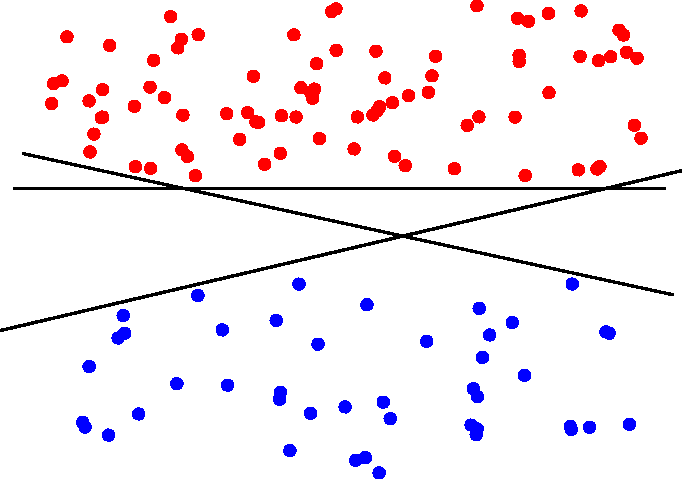
\includegraphics[width=0.5\linewidth]{img/dati_linearmente_separabili.pdf}
    \caption{Esempio di dati linearmente separabili ed alcuni possibili iperpiani di separazione}
    \label{fig:dati_linearmente_separabili}
\end{figure}
Con $\Vec{w}$ e $b$ noti, si definisce il classificatore \[ h(\Vec{x}) = sign(\Vec{w}\cdot \Vec{x} +b). \]
In genere, se i dati sono linearmente separabili, esistono infiniti iperpiani che li separano. Per costruire un buon classificatore, in grado di generalizzare su dati mai visti nella procedura di addestramento, vogliamo identificare l'iperpiano che massimizza il margine di separazione tra le due classi, ovvero l'iperpiano che massimizza la minima distanza tra l'iperpiano stesso ed i punti più vicini di ogni classe. Si definiscono a tale scopo i vincoli 
\begin{equation*}
    \Vec{w}\Vec{x}_i + b \geq M \quad se \quad y_i = +1 \quad  i=1,\dots,m
\end{equation*}
\begin{equation*}
    \Vec{w}\Vec{x}_i + b \leq -M \quad se \quad y_i = -1 \quad i=1,\dots,m
\end{equation*}
che forzano il margine ad essere equidistante dagli iperpiani su cui giacciono i punti più vicini di ogni classe.
Dividendo entrambi i lati delle disequazioni per $M$
\begin{equation*}
\frac{1}{M}\Vec{w}\Vec{x}_i + \frac{1}{M}b \geq 1
\end{equation*}
\begin{equation*}
\frac{1}{M}\Vec{w}\Vec{x}_i + \frac{1}{M}b \leq -1
\end{equation*}
consideriamo l'iperpiano $\frac{1}{M}\Vec{w}\Vec{x}_i + \frac{1}{M}b$ che è equivalente a $\Vec{w}\Vec{x}_i + b$. Il parametro $M$ è quindi in genere fissato ad $1$.
Dato che $y_i\in\{-1,1\}$, i vincoli precedenti possono essere combinati in
\begin{equation*}
    y_i(\Vec{w}\Vec{x}_i + b) \geq 1 \quad i=1, ..., m.
\end{equation*}

L'iperpiano ottimo $\Vec{w}^*\Vec{x} + b^* = 0$ è l'iperpiano che separa linearmente $\mathcal{X}$ massimizzando il margine di separazione, ovvero la distanza tra l'iperpiano ed i punti più vicini per ogni classe. Tali punti, chiamati vettori di supporto, si trovano esattamente sugli iperpiani $\Vec{w}^*\Vec{x} + b^* = \pm 1$. I vettori di supporto definiscono il margine di separazione: se rimuovessimo tutti i punti che non sono vettori di supporto e ripetessimo l'addestramento (con gli stessi iperparametri), otterremmo lo stesso iperpiano.
\begin{figure}
    \centering
    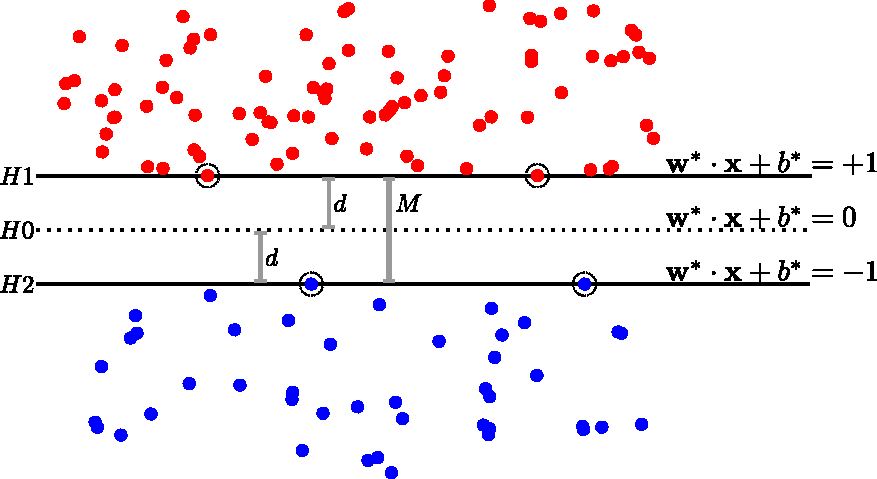
\includegraphics[width=0.7\linewidth]{img/margine_separazione.pdf}
    \caption{Esempio margine di separazione massimale per dati in due dimensioni. I punti cerchiati sono vettori di supporto.}
    \label{fig:optimal_separation_margin}
\end{figure}
%
La distanza tra $\Vec{w}\Vec{x}_i + b = 1$ e $\Vec{w}\Vec{x}_i + b = -1$ è $\frac{2}{\norm{\Vec{w}}}$: massimizzarla equivale a minimizzare $\norm{\Vec{w}}$. Per trovare il margine di separazione massimale, serve quindi risolvere il problema di ottimizzazione
%
\begin{equation}
\label{eq:svc:hardmargin:primal}
\begin{aligned}
& \min_{\Vec{w},b} && \norm{\Vec{w}} \\
& \textrm{s.t.} && y_i(\Vec{w}\cdot \Vec{x}_i + b) \geq 1 && i=1,\dots,m. \\
\end{aligned}
\end{equation}
%
Il problema~\cref{eq:svc:hardmargin:primal} ha funzione obiettivo quadratica e vincoli lineari. I modelli ottenuti risolvendo questo problema sono chiamati \emph{hard margin} perché non ammettono la presenza di anomalie nei dati: tutti gli esempi della stessa classe devono necessariamente essere nello stesso semispazio identificato dal margine. La~\cref{sec:soft_margin_classifier} presenterà la formulazione \emph{soft margin}, che tollera dati anomali (ma ne subisce comunque gli effetti negativi). 


\subsection{Formulazione duale}\label{subsec:hard_margin_dual}
Per convenienza, riscriviamo la funzione obiettivo del problema primale~\cref{eq:svc:hardmargin:primal} ed esprimiamo i vincoli in forma normale.
\begin{equation}\label{eq:svc:hardmargin:primal_convenient}
\begin{aligned}
& \min_{\Vec{w},b}    && \frac{1}{2}\norm{\Vec{w}}^2 \\
& \textrm{s.t.} && y_i(\Vec{w}\cdot \Vec{x}_i + b) - 1 \geq 0 && i=1,\dots,m \\
\end{aligned}
\end{equation}
%
Applichiamo il metodo dei moltiplicatori di Lagrange e otteniamo la funzione lagrangiana
\begin{equation}
\label{eq:svc:hardmargin:lagrangian}
\begin{split}
L_P(\Vec{w},b, \alpha)  & = \frac{1}{2}\norm{\Vec{w}}^2 - \sum_{i=1}^{m} \alpha_i [y_i(\Vec{w}\cdot \Vec{x}_i +b) -1] =\\
        & = \frac{1}{2}\sqrt{\Vec{w} \cdot \Vec{w}}^2 - \sum_{i=1}^{m} \alpha_i y_i(\Vec{w}\cdot \Vec{x}_i +b) -  \sum_{i=1}^{m} - \alpha_i = \\
        & = \frac{1}{2}\Vec{w}\cdot\Vec{w} - \sum_{i=1}^{m} \alpha_i y_i \Vec{w}\cdot \Vec{x}_i - b \sum_{i=1}^{m} \alpha_i y_i + \sum_{i=1}^{m} \alpha_i 
\end{split}
\end{equation}
da minimizzare rispetto a $\Vec{w},b$ e massimizzare rispetto ad $\alpha$ 
\begin{equation}
\label{eq:svc:hardmargin:max_min}
\begin{aligned}
& \max_{\alpha} \min_{\Vec{w}, b} && L_P(\Vec{w},b, \alpha) \\
& \textrm{s.t.} && \alpha_i \geq 0 && i=1,..., m.\\
\end{aligned}
\end{equation}
%
%
Una soluzione ottima per il problema~\cref{eq:svc:hardmargin:max_min} deve soddisfare le condizioni di Karush-Kuhn-Tucker (KKT):
\begin{align}
    \label{eq:svc:hardmargin:kkt1}
    \pd{L_P(\Vec{w},b,\alpha)}{\Vec{w}} = \Vec{0}, \\[2mm]
    \label{eq:svc:hardmargin:kkt2}
    \pd{L_P(\Vec{w},b,\alpha)}{b} = 0, 
\end{align}
\begin{align}
    \label{eq:svc:hardmargin:kkt3}
    y_i(\Vec{x}_i\cdot\Vec{w}+b)-1 \geq 0 && i=1,\dots,m,  \\[2mm]
    \label{eq:svc:hardmargin:kkt4}
    \alpha_i \geq 0 && i=1,\dots,m,  \\[2mm]
    \label{eq:svc:hardmargin:kkt5}
    \alpha_i[y_i(\Vec{x}_i\cdot\Vec{w}+b)-1] = 0  && i=1,\dots,m.
\end{align}
%Il problema~\ref{eq:svc:hardmargin:max_min} è quadratico convesso **fidatevi**.
%
Le condizioni~\cref{eq:svc:hardmargin:kkt1,eq:svc:hardmargin:kkt2}
\begin{align*}
    \pd{L_P}{\Vec{w}} &= \Vec{w} - \sum_{i=1}^{m}\alpha_iy_i\Vec{x_i} = 0\\
    \pd{L_P}{b} &=  \sum_{i=1}^{m}\alpha_iy_i =0
\end{align*}
si riducono a
\begin{equation}
\label{eq:svc_sub1}
\Vec{w} = \sum_{i=1}^{m}\alpha_iy_i\Vec{x}_i
\end{equation}
\begin{equation}
\label{eq:svc_sub2}
\sum_{i=1}^{m}\alpha_iy_i = 0.
\end{equation}
% representer theorem [Kimeldorf and Wahba,1971] tells us that the optimal solution w∗ of the primal problem can be represented as a linear combination
Sostituendo~\cref{eq:svc_sub1,eq:svc_sub2} nella funzione~(\ref{eq:svc:hardmargin:lagrangian}), 
otteniamo la funzione obiettivo duale
\begin{equation}
\label{eq:svc:hardmargin:dual_obj_fn}
\begin{split}
L_D(\alpha)  & = \frac{1}{2}\Vec{w}\cdot\Vec{w} - \sum_{i=1}^{m} \alpha_i y_i \Vec{w}\cdot \Vec{x}_i - b \sum_{i=1}^{m} \alpha_i y_i + \sum_{i=1}^{m} \alpha_i =\\
 &= \frac{1}{2}\sum_{i=1}^{m}\alpha_iy_i\Vec{x_i} \cdot \sum_{i=1}^{m}\alpha_iy_i\Vec{x_i} - \sum_{i=1}^{m} \alpha_i y_i \Vec{x}_i \sum_{j=1}^{m}\alpha_jy_j\Vec{x_j} + \sum_{i=1}^{m} \alpha_i =\\
 &= \frac{1}{2}\sum_{i=1}^{m}\sum_{j=1}^{m}\alpha_i\alpha_jy_iy_j\Vec{x}_i\cdot\Vec{x}_j - 
 \sum_{i=1}^{m}\sum_{j=1}^{m}\alpha_i\alpha_jy_iy_j\Vec{x}_i\cdot\Vec{x}_j + \sum_{i=1}^{m} \alpha_i =\\
 &= -\frac{1}{2}\sum_{i=1}^{m}\sum_{j=1}^{m}\alpha_i\alpha_jy_iy_j\Vec{x}_i\cdot\Vec{x}_j + \sum_{i=1}^{m} \alpha_i 
\end{split}  
\end{equation}
espressa esclusivamente in funzione di $\alpha$.
Aggiungendo i rimanenti vincoli, otteniamo la formulazione del problema duale
\begin{equation}\label{eq:svc:hardmargin:wolfe_dual}
\begin{aligned}
& \max_{\alpha}     && \sum_{i=1}^{m}\alpha_i - \frac{1}{2}\sum_{i=1}^{m}\sum_{j=1}^{m}\alpha_i\alpha_jy_iy_j\Vec{x}_i\cdot\Vec{x}_j\\
& \textrm{s.t.}     && \sum_{i=1}^{m} \alpha_iy_i = 0 \\
&                   && \alpha_i \geq 0 && i=1,\dots,m. \\
\end{aligned}
\end{equation}
%
Una volta risolto il problema duale~\cref{eq:svc:hardmargin:wolfe_dual} all'ottimo, avremo i moltiplicatori lagrangiani $\alpha_1^*, ..., \alpha_m^*$.
Ricordando che $\Vec{w} = \sum_{i=1}^{m}\alpha_iy_i\Vec{x}_i$, possiamo calcolare l'ottimo 
\begin{equation}\label{eq:representer_w} %??
\Vec{w}^* = \sum_{i=1}^{m}\alpha_i^*y_i\Vec{x}_i.
\end{equation}
$\Vec{w}^*$ è definito dai i dati di addestramento $\Vec{x}_i$ con un corrispettivo moltiplicatore lagrangiano $\alpha_i > 0$: i vettori di supporto. 
Il risultato in~\cref{eq:representer_w} è generalizzato per altri metodi kernel dal \emph{representer theorem}. Il teorema, nel contesto di alcuni problemi con funzioni kernel, afferma che la soluzione ottima può essere rappresentata come combinazione lineare di funzioni kernel calcolate su alcuni dati di addestramento. 
In generale, possiamo inserire i modelli SVC nella categoria degli \emph{instance based learner}, dato che eseguono predizioni utilizzando un sottoinsieme dei dati di addestramento.

Per costruire il classificatore $h(\Vec{x}) = sign(\Vec{w}\cdot \Vec{x} +b)$, dobbiamo ancora ricavare $b$.  Dalla condizione di KKT~\cref{eq:svc:hardmargin:kkt5}, la soluzione ottima soddisferà il vincolo 
\begin{equation*}
\alpha_i(y_i(\Vec{w}^*\cdot\Vec{x}_i+b^*)-1)=0.
\end{equation*}
Per gli $\alpha_i > 0$, rispettare il vincolo significa rispettare 
\begin{equation*}
y_i(\Vec{w}^*\cdot\Vec{x}_i+b^*) -1 = 0.
\end{equation*}
Dato che $y_i \in \{-1,1\}$, possiamo semplificare in 
\begin{equation*}
\Vec{w}^*\cdot\Vec{x}_i+b^*=y_i
\end{equation*}
ottenendo 
\begin{equation*}
b^*=y_i - \Vec{w}^*\cdot\Vec{x}_i.
\end{equation*} 
Nella pratica, per ottenere un valore numericamente più stabile, si calcola la media tra ogni $b^*$ calcolato su ogni vettore di supporto.

Ricapitolando, risolvendo il problema duale~\cref{eq:svc:hardmargin:wolfe_dual}, che contiene meno variabili del problema primale e che può essere risolto con varie tecniche note, otteniamo i moltiplicatori lagrangiani ottimi $\alpha_1^*, ..., \alpha_m^*$ che consentono di calcolare $\Vec{w}^*$ come combinazione lineare tra i vettori di supporto ed in seguito calcolare $b^*$. 
Tutti gli altri dati di addestramento non influiscono sulla soluzione. 
A questo punto, è costruito il classificatore $h(\Vec{x}) = sign(\Vec{w}^*\cdot \Vec{x} +b^*)$.
La predizione della classe di un nuovo esempio $\Vec{x}_{test}$ sarà ottenuta calcolando 
\begin{equation*}
\begin{aligned}
& h(\Vec{x}_{test}) = sign\left(\sum_{i=1}^{m}\alpha_i^*y_i\Vec{x}_i \cdot \Vec{x}_{test} + b^*\right) & \forall i | \alpha_i > 0
\end{aligned}
\end{equation*}



\section{Classificazione \emph{soft margin}}\label{sec:soft_margin_classifier}
La formulazione \emph{hard margin} funziona solo su dati linearmente separabili, il che rende il modello troppo rigido per essere applicato su dataset tratti da problemi reali, che spesso esibiscono relazioni più complesse. 
Anche nel caso di dati linearmente separabili, un modello \emph{hard margin} potrebbe esibire cattive capacità di generalizzazione a causa di un margine negativamente influenzato da pochi dati erroneamente classificati.
Si riportano due esempi di questi scenari in~\cref{fig:svc:softmargin:casi_che_hardmargin_non_risolve}.

\begin{figure}[ht]
    \centering
    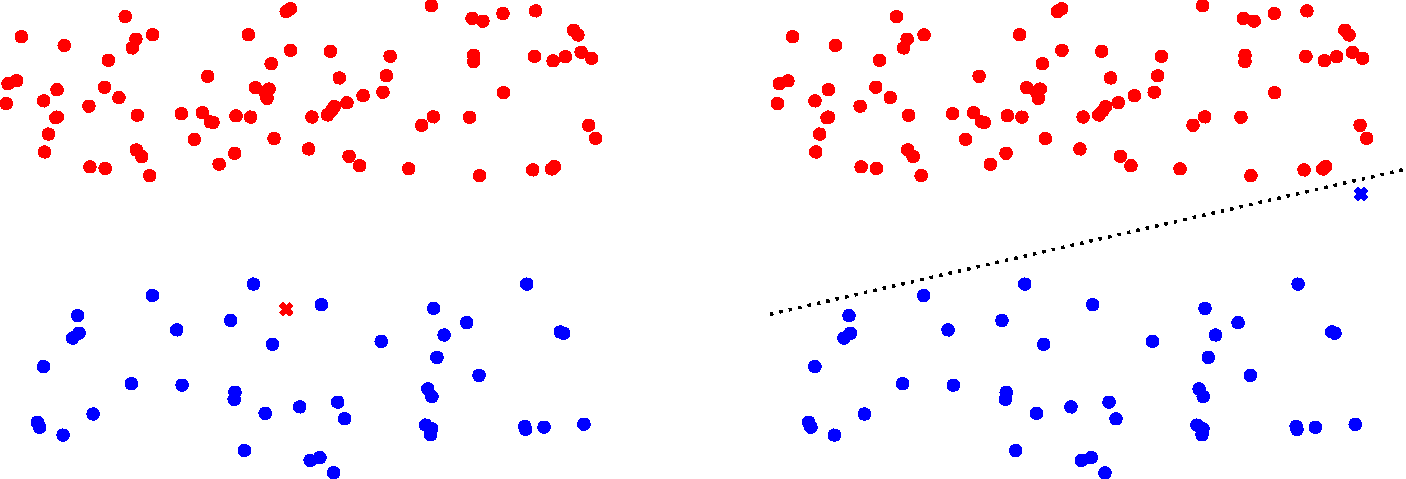
\includegraphics[width=\linewidth]{img/casi_dove_hardmargin_va_male_o_non_va.pdf}
    \caption{A sinistra un esempio di dataset non linearmente separabile, non risolvibile con il modello \emph{hard margin}. A destra un caso linearmente separabile la cui soluzione \emph{hard margin} è pesantemente influenzata da un \emph{outlier}.}
    \label{fig:svc:softmargin:casi_che_hardmargin_non_risolve}
\end{figure}
Per generalizzare il modello \emph{support vector classifier} e renderlo tollerante ad errori di classificazione, si riformula il problema di ottimizzazione, introducendo le variabili di \emph{slack} $\xi_i \geq 0 \quad i=1,...,m$, una per ogni dato di addestramento. Ogni valore $\xi_i$ sarà proporzionale alla distanza tra $\Vec{x}_i$ erroneamente classificato ed il margine. $\xi_i$ sarà nulla per ogni $\Vec{x}_i$ correttamente classificato. Resta da definire come utilizzare le variabili di \emph{slack} per penalizzare la scelta di dati erroneamente classificati. 
In generale si ottiene il problema primale
\begin{equation}
\begin{aligned}
& \min_{\Vec{w},b}    && \norm{\Vec{w}} + \frac{C}{p}\sum_{i=1}^{m}\xi_i^p\\
& \textrm{s.t.} && y_i(\Vec{w}\cdot\Vec{x}_i + b) \geq 1 - \xi_i &&  i=1,\dots,m \\
&               && \xi_i \geq 0                 &&  i=1,\dots,m.\\
\end{aligned}
\end{equation}
Il parametro $C$, fissato a priori, determina il grado di tolleranza agli \emph{outlier}, bilanciando la funzione obiettivo originale con la penalità introdotta dalle variabili di \emph{slack}.
%
Il valore di $p$ è in genere uguale a $1$ (L1-SVC) oppure $2$ (L2-SVC). Consideriamo la più semplice formulazione L1-SVC:
\begin{equation}
\label{eq:svc:softmargin:primal}
\begin{aligned}
& \min_{\Vec{w},b}    && \norm{\Vec{w}} + C\sum_{i=1}^{m}\xi_i\\
& \textrm{s.t.} && y_i(\Vec{w}\cdot\Vec{x}_i + b) \geq 1 - \xi_i &&  i=1,\dots,m \\
&               && \xi_i \geq 0                 &&  i=1,\dots,m.\\
\end{aligned}
\end{equation}
Il modello così modificato, viene chiamato \emph{soft margin support vector classifier}.
\begin{figure}[ht]
    \centering
    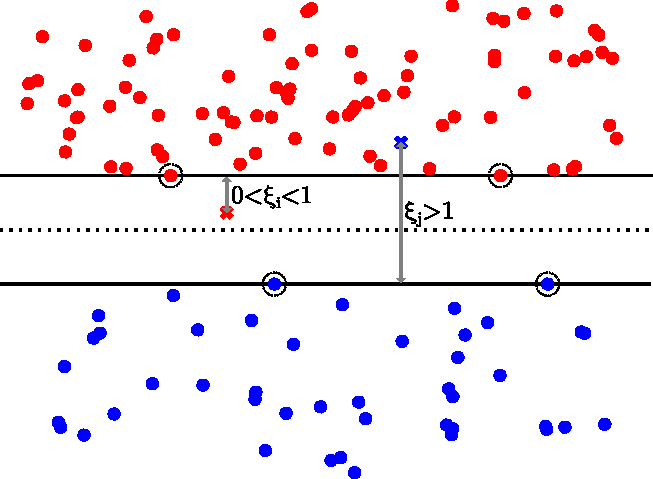
\includegraphics[width=.7\linewidth]{img/soft_margin.pdf}
    \caption{Con la formulazione \emph{soft margin} si tollerano esempi dalla parte sbagliata del margine o troppo vicini al margine}
    \label{fig:soft_margin}
\end{figure}



\subsection{Formulazione duale}\label{subsec:soft_margin_dual}
Il procedimento per ricavare la formulazione duale è analogo al caso \emph{hard margin}.
Riscriviamo la funzione obiettivo del problema~\cref{eq:svc:softmargin:primal} ed esprimiamo i vincoli in forma normale.
\begin{equation}
\label{eq:svc:softmargin:primal_convenient}
\begin{aligned}
& \min_{w,b}    && \frac{1}{2}\norm{\Vec{w}}^2 + C\sum_{i=0}^{m} \xi_i \\
& \textrm{s.t.} && y_i(\Vec{w}\cdot \Vec{x}_i + b) - 1 + \xi_i \geq 0 && i=1,\dots,m \\
&               && \xi_i \geq 0  && i=1,\dots,m 
\end{aligned}
\end{equation}
%
Applichiamo il metodo dei moltiplicatori di Lagrange e otteniamo la funzione lagrangiana
\begin{equation}
\label{eq:svc:softmargin:lagrange_fn}
\begin{split}
L_P(\Vec{w},b, \xi_i, \alpha_i, \mu_i) = & \frac{1}{2}\norm{\Vec{w}}^2 + C\sum_{i=0}^{m} \xi_i - \sum_{i=1}^{m} \alpha_i [y_i(\Vec{w}\cdot \Vec{x}_i +b) -1 +\xi_i] - \sum_{i=1}^{m}\mu_i\xi_i =\\
        = & \frac{1}{2}\Vec{w}\cdot\Vec{w} + C\sum_{i=0}^{m} \xi_i - \sum_{i=1}^{m} \alpha_i y_i(\Vec{w}\cdot \Vec{x}_i +b) -  \sum_{i=1}^{m} - \alpha_i  \\ & - \sum_{i=1}^{m} \alpha_i\xi_i - \sum_{i=1}^{m}\mu_i\xi_i= \\
        = & \frac{1}{2}\Vec{w}\cdot\Vec{w} + C\sum_{i=0}^{m} \xi_i - \sum_{i=1}^{m} \alpha_i y_i \Vec{w}\cdot \Vec{x}_i - b \sum_{i=1}^{m} \alpha_i y_i \\ & + \sum_{i=1}^{m} \alpha_i - \sum_{i=1}^{m} \alpha_i\xi_i - \sum_{i=1}^{m}\mu_i\xi_i
\end{split}
\end{equation}
da minimizzare rispetto a $\Vec{w},b,\xi_i$ e massimizzare rispetto ad $\alpha, \mu$ 
\begin{equation}
\label{eq:svc:softmargin:max_min}
\begin{aligned}
& \max_{\alpha, \mu} \min_{\Vec{w}, b, \xi} && L_P(\Vec{w},b, \xi, \alpha, \mu) \\
& \textrm{s.t.} && \alpha_i \geq 0  && i=1,..., m.\\
&               && \mu_i \geq 0     && i=1,..., m.\\
\end{aligned}
\end{equation}
%
Una soluzione ottima per il problema~\cref{eq:svc:softmargin:max_min} deve soddisfare le condizioni di Karush-Kuhn-Tucker:
\begin{align}
    \label{eq:svc:softmargin:kkt1}
    \pd{L_P(\Vec{w},b, \Vec{\xi}, \Vec{\alpha}, \Vec{\mu})}{\Vec{w}} = \Vec{0}  \\[2mm]
    \label{eq:svc:softmargin:kkt2}
    \pd{L_P(\Vec{w},b, \Vec{\xi}, \Vec{\alpha}, \Vec{\mu})}{b} = 0 \\[2mm]
    \label{eq:svc:softmargin:kkt3}
    \pd{L_P(\Vec{w},b, \Vec{\xi}, \Vec{\alpha}, \Vec{\mu})}{\xi} = 0 
\end{align}
\begin{align}
    \label{eq:svc:softmargin:kkt4}
    \alpha_i[y_i(\Vec{x}_i\cdot\Vec{w}+b)-1+\xi_i] = 0  && i=1,\dots,m \\[2mm] 
    \label{eq:svc:softmargin:kkt5}
    \mu_i\xi_i = 0 && i=1,\dots,m \\[2mm] 
    \label{eq:svc:softmargin:kkt6}
    \alpha_i \geq 0, \mu_i \geq 0, \xi_i \geq 0 && i=1,\dots,m
\end{align}
Le condizioni~\cref{eq:svc:softmargin:kkt1,eq:svc:softmargin:kkt2,eq:svc:softmargin:kkt3}
\begin{equation*}
    \begin{split}
        \pd{L}{\Vec{w}} & = \Vec{w} - \sum_{i=1}^{m}\alpha_iy_i\Vec{x_i} = 0\\
        \pd{L}{b} &=  \sum_{i=1}^{m}\alpha_iy_i = 0\\
        \pd{L}{\xi_i} &= C -\sum_{i=1}^{m}\alpha_i - \sum_{i=1}^{m}\mu_i = 0
    \end{split}
\end{equation*}
si riducono a
\begin{align} 
    \label{eq:svc_hard_sub1}
    \Vec{w} = \sum_{i=1}^{m}\alpha_iy_i\Vec{x}_i  \\[2mm]
    \label{eq:svc_hard_sub2}
    \sum_{i=1}^{m}\alpha_iy_i = 0 \\[2mm]
    \label{eq:svc_hard_sub3}
    C = \sum_{i=1}^{m}\alpha_i + \sum_{i=1}^{m}\mu_i.
\end{align}
Sostituendo~\cref{eq:svc_hard_sub1,eq:svc_hard_sub2,eq:svc_hard_sub3} in~\cref{eq:svc:softmargin:lagrange_fn} otteniamo la funzione obiettivo duale
\begin{equation}
\begin{split}
L_D(\Vec{w},b, \xi_i, \alpha_i, \mu_i) = & \frac{1}{2}\Vec{w}\cdot\Vec{w} + C\sum_{i=0}^{m} \xi_i - \sum_{i=1}^{m} \alpha_i y_i \Vec{w}\cdot \Vec{x}_i - b \sum_{i=1}^{m} \alpha_i y_i \\ & + \sum_{i=1}^{m} \alpha_i - \sum_{i=1}^{m} \alpha_i\xi_i - \sum_{i=1}^{m}\mu_i\xi_i =\\
= & \frac{1}{2}\sum_{i=1}^{m}\alpha_iy_i\Vec{x}_i \cdot \sum_{i=1}^{m}\alpha_iy_i\Vec{x}_i  + \sum_{i=1}^{m}\alpha_i\xi_i + \sum_{i=1}^{m}\mu_i\xi_i \\
& - \sum_{i=1}^{m} \alpha_i y_i  \cdot \Vec{x}_i \sum_{j=1}^{m}\alpha_jy_j\Vec{x}_j + \sum_{i=1}^{m} \alpha_i - \sum_{i=1}^{m} \alpha_i\xi_i - \sum_{i=1}^{m}\mu_i\xi_i =\\
=& \frac{1}{2}\sum_{i=1}^{m}\sum_{j=1}^{m}\alpha_i\alpha_jy_iy_j\Vec{x}_i\cdot\Vec{x_j} + \sum_{i=1}^{m} \alpha_i
\end{split}  
\end{equation}
espressa esclusivamente in funzione di $\alpha$.
Aggiungendo i rimanenti vincoli, otteniamo la formulazione del problema duale
\begin{equation}\label{eq:svc:softmargin:wolfe_dual}
\begin{aligned}
& \max_{\alpha}    && \sum_{i=1}^{m}\alpha_i - \frac{1}{2}\sum_{i=1}^{m}\sum_{j=1}^{m}\alpha_i\alpha_jy_iy_j\Vec{x}_i\cdot\Vec{x}_j\\
& \textrm{s.t.} && \sum_{i=1}^{m} \alpha_iy_i = 0 \\
&               && 0 \leq \alpha_i \leq C && i=1,\dots,m. \\
\end{aligned}
\end{equation}
Come nel caso soft margin, $\Vec{w}^*$ e $b^*$ sono ricavati dai vettori di supporto.
Si può notare come la formulazione duale \emph{hard margin} sia sostanzialmente identica alla formulazione duale \emph{soft margin}, con la differenza che in quest'ultima i moltiplicatori lagrangiani hanno un valore limitato al massimo a $C$.

% Dimitris Bertsimas, Jack Dunn, Colin Pawlowski, Ying Daisy Zhuo (2019) Robust Classification. INFORMS Journal on Optimization 1(1):2-34. https://doi.org/10.1287/ijoo.2018.0001 '' Both the primal and dual are convex quadratic optimization problems. Because the dual problem has fewer decision variables, and the majority of these variables tend to be equal to zero or the cost parameter C in the optimal solution, it is typically the problem solved in practice (Friedman et al. 2001). In addition, the dual form is ad vantageous because it allows us to do the kernel trick to learn nonlinear decision rules (Cortes and Vapnik 1995).''



\section{\emph{Kernel trick}}\label{sec:kernel_trick}
I modelli visti fino ad ora, sono dei classificatori lineari e non sono in grado di modellare relazioni più intricate.
Come anticipato in~\cref{sec:kernel_methods}, si può rendere il modello non lineare utilizzando una funzione kernel.
Si potrebbero processare i dati prima di addestrare un modello, applicando una trasformazione in grado di renderli linearmente separabili.
\begin{figure}[ht]
    \centering
    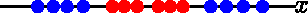
\includegraphics[width=0.5\linewidth]{img/non_linearmente_separabili.pdf}
    \caption{Esempio in una dimensione di dati non linearmente separabili}
    \label{fig:kerneltrick:non_lin_sep}
\end{figure}
Consideriamo l'esempio mostrato in~\cref{fig:kerneltrick:non_lin_sep}, dove i dati in uno spazio monodimensionale, non sono linearmente separabili. Ipotizziamo di trasformarli utilizzando la mappatura $\Phi:\mathbb{R} \rightarrow \mathbb{R}^2$ con $\Phi(x) = (x, x^2)$. Otterremmo un dataset, visualizzato in~\cref{fig:kerneltrick:visualized}, che nel nuovo spazio è linearmente separabile.
\begin{figure}[ht]
    \centering
    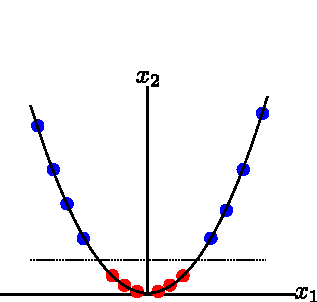
\includegraphics[width=0.5\linewidth]{img/kernel_trick_visualized.pdf}
    \caption{I dati trasformati sono linearmente separabili}
    \label{fig:kerneltrick:visualized}
\end{figure}

In generale, vorremmo mappare i dati di addestramento dallo spazio originale $\mathcal{X}$ ad un altro spazio $\mathcal{H}$ di dimensioni maggiori, potenzialmente infinite, usando una mappatura
\begin{equation}
\label{eq:generic_kernel_mapping}
\Phi(x_i) : \mathcal{X} \rightarrow \mathcal{H}
\end{equation}
in modo da rendere i dati linearmente separabili in $\mathcal{H}$.
%
%
Come si integra questa trasformazione dei dati nella procedura di addestramento? Rifacendosi alla formulazione del problema~\ref{eq:svc:softmargin:wolfe_dual}, i dati di addestramento compaiono nella funzione obiettivo come prodotto scalare tra di essi. Se volessimo applicare la trasformazione $\Phi$, dovremmo dunque calcolare $\Phi(\Vec{x}_i)\cdot\Phi(\Vec{x}_j)$ per $i=1,\dots,m$, il che renderebbe la procedura costosa dal punto di vista computazionale, se non impossibile ($\mathcal{H}$ di infinite dimensioni). Il \emph{kernel trick}, consiste nell'utilizzare una funzione 
$$K(\Vec{x}_i, \Vec{x}_j) = \Phi(\Vec{x}_i)\cdot\Phi(\Vec{x}_j),$$ in modo che la mappatura $\Phi$ non debba essere calcolata esplicitamente. Il \emph{kernel} ritorna direttamente il prodotto scalare tra i punti trasformati, senza effettivamente trasformarli. Il valore $K(\Vec{x_i}, \Vec{x_j})$ può essere interpretato come una misura della ``distanza'' tra i punti $\Vec{x_i}, \Vec{x_j}$.
Esistono diversi kernel, i più utilizzati sono riportati nell'elenco seguente.
\begin{itemize}
    \item Lineare: $K(\Vec{x}_1, \Vec{x}_2) = \Vec{x}_1\cdot\Vec{x}_2$.
    \item Polinomiale: $K(\Vec{x}_1, \Vec{x}_2) = (\Vec{x}_1\cdot\Vec{x}_2 + \gamma)^d$.
    \item Gaussiano: $K(\Vec{x}_1, \Vec{x}_2) = exp({-\frac{\norm{\Vec{x}_1 - \Vec{x}_2}^2}{2 \sigma^2}})$.
\end{itemize}
%
In generale, le condizioni per far si che una funzione $K$ sia un \emph{kernel}, derivano dal teorema di Mercer. Se la funzione \emph{kernel} $K$ è simmetrica, continua e definita semi-positiva, allora esiste una funzione $\Phi(x) : \mathbb{R}^p \rightarrow \mathcal{H}$ tale per cui $K(\Vec{x}_i, \Vec{x}_j) = \Phi(\Vec{x}_i)\cdot\Phi(\Vec{x}_j)$. 

L'introduzione del \emph{kernel trick} modifica il problema~(\ref{eq:svc:softmargin:wolfe_dual}), che diventa quindi
\begin{equation}\label{eq:svc:softmargin:wolfe_dual_plus_kernel_trick}
\begin{aligned}
& \max_{\alpha}    && \sum_{i=1}^{m}\alpha_i - \frac{1}{2}\sum_{i=1}^{m}\sum_{j=1}^{m}\alpha_i\alpha_jy_iy_jK(\Vec{x}_i, \Vec{x}_j)\\
& \textrm{s.t.} && \sum_{i=1}^{m} \alpha_iy_i = 0 \\
&               && 0 \leq \alpha_i \leq C && i=1,\dots,m. \\
\end{aligned}
\end{equation}
%
La predizione della classe di un nuovo esempio $\Vec{x}_{test}$ sarà ottenuta calcolando 
\begin{equation*}
\begin{aligned}
& h(\Vec{x}_{test}) = sign\left(\sum_{i=1}^{m}\alpha_i^*y_iK(\Vec{x}_i, \Vec{x}_{test}) + b^*\right) & \forall i | \alpha_i \neq 0.
\end{aligned}
\end{equation*}

In uno spazio con più dimensioni rispetto all'originale, è spesso possibile trovare un margine di separazione in grado di dividere i dati delle due classi perfettamente. Pur essendo un risultato più preciso dal punto di vista del problema di ottimizzazione, si tratta in realtà di \emph{overfitting}. Rimane dunque cruciale la scelta del parametro $C$. Per un $C$ troppo alto, il modello cercherà di adattarsi troppo fedelmente ai dati di addestramento, creando un margine inutilmente contorto e con pessime capacità di generalizzazione. Al contrario, un valore basso di $C$ porterà ad un margine più semplice. Per trovare un valore di $C$ soddisfacente, si utilizzano delle tecniche di model selection.  



\section{Limitazioni}\label{sec:svc_limiti}
I \emph{support vector classifier} presentano alcune limitazioni di cui serve tener conto. 
Sono modelli suscettibili alla presenza di \emph{outlier}, intesi come dati erroneamente classificati o rumore. L'approccio \emph{soft-margin} consente di trattare anche problemi di questo tipo, ma la soluzione trovata subirà comunque l'effetto degli \emph{outlier}, dato che ognuno di questi punti diventerà un vettore di supporto con una relativa variabile di \emph{slack} che influirà sul valore della funzione obiettivo. Di conseguenza, i modelli SVC addestrati su dataset con rumore hanno in genere performance peggiori rispetto ad altri tipi di modelli. 

Una seconda limitazione riguarda la scalabilità. La procedura di addestramento considera tutti i dati disponibili e risulta quindi troppo costosa da eseguire su grandi quantità di dati, o su dati con un alto numero di feature, pur utilizzando un algoritmo risolutivo efficiente, come \emph{sequential minimal optimization} \cite{SMO}.

Una terza limitazione riguarda la selezione dei parametri di addestramento: il costo $C$ e la funzione kernel. La scelta ottimale di questi valori richiede in genere molteplici esecuzioni dell'algoritmo di addestramento, moltiplicando i tempi necessari.

Risultano motivati dunque tutti gli approcci che tentano di risolvere queste limitazioni. 

